% This file was created with tikzplotlib v0.9.12.
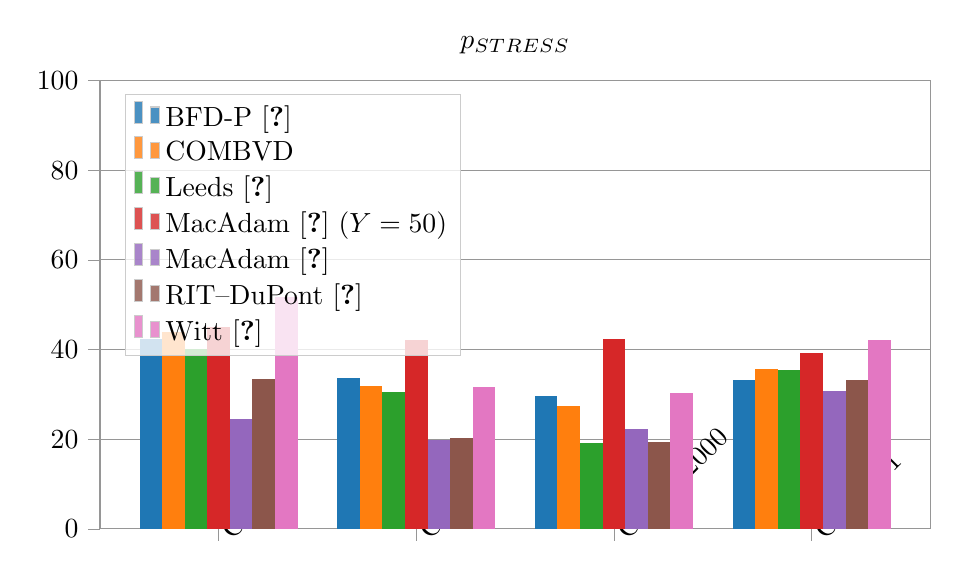
\begin{tikzpicture}

\definecolor{color0}{rgb}{0.12156862745098,0.466666666666667,0.705882352941177}
\definecolor{color1}{rgb}{1,0.498039215686275,0.0549019607843137}
\definecolor{color2}{rgb}{0.172549019607843,0.627450980392157,0.172549019607843}
\definecolor{color3}{rgb}{0.83921568627451,0.152941176470588,0.156862745098039}
\definecolor{color4}{rgb}{0.580392156862745,0.403921568627451,0.741176470588235}
\definecolor{color5}{rgb}{0.549019607843137,0.337254901960784,0.294117647058824}
\definecolor{color6}{rgb}{0.890196078431372,0.466666666666667,0.76078431372549}

\begin{axis}[
axis line style={white!58.8235294117647!black},
height=0.6\textwidth,
legend cell align={left},
legend style={
  fill opacity=0.8,
  draw opacity=1,
  text opacity=1,
  at={(0.03,0.97)},
  anchor=north west,
  draw=white!80!black
},
tick align=outside,
tick pos=left,
title={\(\displaystyle p_{STRESS}\)},
width=\textwidth,
x grid style={white!58.8235294117647!black},
xmin=-0.6, xmax=3.6,
xtick style={color=white!58.8235294117647!black},
xtick={0,1,2,3},
xticklabel style={rotate=45.0,anchor=west},
xticklabels={CIE76,CIE94,CIEDE2000,CMC 2:1},
y grid style={white!58.8235294117647!black},
ymajorgrids,
ymin=0, ymax=100,
ytick style={color=white!58.8235294117647!black}
]
\draw[draw=none,fill=color0] (axis cs:-0.4,0) rectangle (axis cs:-0.285714285714286,42.4625947678848);
\addlegendimage{ybar,ybar legend,draw=none,fill=color0}
\addlegendentry{BFD-P \cite{luorigg}}

\draw[draw=none,fill=color0] (axis cs:0.6,0) rectangle (axis cs:0.714285714285714,33.704333992779);
\draw[draw=none,fill=color0] (axis cs:1.6,0) rectangle (axis cs:1.71428571428571,29.5541899707267);
\draw[draw=none,fill=color0] (axis cs:2.6,0) rectangle (axis cs:2.71428571428571,33.1843269563939);
\draw[draw=none,fill=color1] (axis cs:-0.285714285714286,0) rectangle (axis cs:-0.171428571428571,43.9286196626574);
\addlegendimage{ybar,ybar legend,draw=none,fill=color1}
\addlegendentry{COMBVD}

\draw[draw=none,fill=color1] (axis cs:0.714285714285714,0) rectangle (axis cs:0.828571428571429,31.9307958569976);
\draw[draw=none,fill=color1] (axis cs:1.71428571428571,0) rectangle (axis cs:1.82857142857143,27.4886833666082);
\draw[draw=none,fill=color1] (axis cs:2.71428571428571,0) rectangle (axis cs:2.82857142857143,35.5734215522358);
\draw[draw=none,fill=color2] (axis cs:-0.171428571428571,0) rectangle (axis cs:-0.0571428571428571,40.093223056789);
\addlegendimage{ybar,ybar legend,draw=none,fill=color2}
\addlegendentry{Leeds \cite{leeds}}

\draw[draw=none,fill=color2] (axis cs:0.828571428571429,0) rectangle (axis cs:0.942857142857143,30.494358035554);
\draw[draw=none,fill=color2] (axis cs:1.82857142857143,0) rectangle (axis cs:1.94285714285714,19.2469488498468);
\draw[draw=none,fill=color2] (axis cs:2.82857142857143,0) rectangle (axis cs:2.94285714285714,35.5150605885755);
\draw[draw=none,fill=color3] (axis cs:-0.0571428571428571,0) rectangle (axis cs:0.0571428571428571,44.9543269657765);
\addlegendimage{ybar,ybar legend,draw=none,fill=color3}
\addlegendentry{MacAdam \cite{macadam1942} ($Y=50$)}

\draw[draw=none,fill=color3] (axis cs:0.942857142857143,0) rectangle (axis cs:1.05714285714286,42.1112585972301);
\draw[draw=none,fill=color3] (axis cs:1.94285714285714,0) rectangle (axis cs:2.05714285714286,42.2606719276812);
\draw[draw=none,fill=color3] (axis cs:2.94285714285714,0) rectangle (axis cs:3.05714285714286,39.2053601641461);
\draw[draw=none,fill=color4] (axis cs:0.0571428571428571,0) rectangle (axis cs:0.171428571428571,24.5477402934334);
\addlegendimage{ybar,ybar legend,draw=none,fill=color4}
\addlegendentry{MacAdam \cite{macadam1974}}

\draw[draw=none,fill=color4] (axis cs:1.05714285714286,0) rectangle (axis cs:1.17142857142857,19.7334023705718);
\draw[draw=none,fill=color4] (axis cs:2.05714285714286,0) rectangle (axis cs:2.17142857142857,22.2667940227177);
\draw[draw=none,fill=color4] (axis cs:3.05714285714286,0) rectangle (axis cs:3.17142857142857,30.7788758540828);
\draw[draw=none,fill=color5] (axis cs:0.171428571428571,0) rectangle (axis cs:0.285714285714286,33.4159367334339);
\addlegendimage{ybar,ybar legend,draw=none,fill=color5}
\addlegendentry{RIT--DuPont \cite{berns}}

\draw[draw=none,fill=color5] (axis cs:1.17142857142857,0) rectangle (axis cs:1.28571428571429,20.2995997396571);
\draw[draw=none,fill=color5] (axis cs:2.17142857142857,0) rectangle (axis cs:2.28571428571429,19.469797268868);
\draw[draw=none,fill=color5] (axis cs:3.17142857142857,0) rectangle (axis cs:3.28571428571429,33.2089174911718);
\draw[draw=none,fill=color6] (axis cs:0.285714285714286,0) rectangle (axis cs:0.4,51.7088993571149);
\addlegendimage{ybar,ybar legend,draw=none,fill=color6}
\addlegendentry{Witt \cite{witt}}

\draw[draw=none,fill=color6] (axis cs:1.28571428571429,0) rectangle (axis cs:1.4,31.704895635913);
\draw[draw=none,fill=color6] (axis cs:2.28571428571429,0) rectangle (axis cs:2.4,30.2182343573007);
\draw[draw=none,fill=color6] (axis cs:3.28571428571429,0) rectangle (axis cs:3.4,42.1795697284095);
\end{axis}

\end{tikzpicture}
